%!TEX root = Slic3r-Manual.tex

\section{Contour} % (fold)
\label{sec:skirt}
\index{skirt}
\index{contour}
\index{Print Settings!Skirt and brim!Skirt}
\index{Param\`etres d'Impression!Contour et bordure!Contour}

Le param\`etre \texttt{Skirt} (Contour) ajoute une extrusion \`a une courte distance du perim\`etre de l'objet. Ceci peut faire en sorte que le mat\'eriau sorte de l'extrudeuse correctement, avant de commencer sur le mod\`ele correspondant.

\begin{figure}[H]
\centering
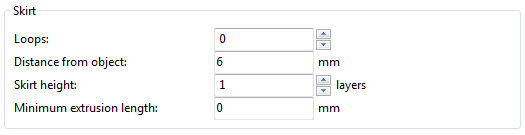
\includegraphics[keepaspectratio=true,width=1.0\textwidth]{expertmode/skirt_settings.png}
\caption{Param\`etres de contour.}
\label{fig:skirt_settings}
\end{figure}

\begin{itemize}
    \index{Print Settings!Skirt and brim!Skirt!Loops}
	\index{Param\`etres d'Impression!Contour et bordure!Contour!Boucles}
    \item \texttt{Loops} (Boucles) - Combien de circuits devraient \^etre achev\'es avant de commencer le mod\`ele. Une boucle est g\'en\'eralement suffisante.
    \index{Print Settings!Skirt and brim!Skirt!Distance from object}
	\index{Param\`etres d'Impression!Contour et bordure!Contour!Distance de l'objet}
    \item \texttt{Distance from object} (Distance de l'objet) - Les millim\`etres entre l'objet et le contour. La valeur par d\'efaut de 6 mm est g\'en\'eralement suffisante.
    \index{Print Settings!Skirt and brim!Skirt!Skirt height}
	\index{Param\`etres d'Impression!Contour et bordure!Contour!Hauteur du contour}
    \item \texttt{Skirt height} (Hauteur du contour) - Le nombre de couches \`a imprimer pour le contour. Pour assurer le mat\'eriau sorte correctement, une couche suffit, mais la fonction de contour peut \'egalement \^etre utilis\'e pour construire des murs autour de l'objet au cas o\`u il devrait \^etre prot\'eg\'e des courants d'air.
    \index{Print Settings!Skirt and brim!Skirt!Minimum extrusion length}
	\index{Param\`etres d'Impression!Contour et bordure!Contour!Longueur minimum d'extrusion}
    \item \texttt{Minimum extrusion length} - Indique le nombre minimum de millim\`etres que le contour doit avoir, si la boucle autour de l'objet ne suffit pas.
\end{itemize}

% section skirt (end)